%%%%%%%%%%%%%%%%%%%%%%%%%%%%%%%%%%%%%%%%%%
% Beamer Presentation
% LaTeX Template
% Version 1.0 (10/11/12)
%
% This template has been downloaded from:
% http://www.LaTeXTemplates.com
%
% License:
% CC BY-NC-SA 3.0 (http://creativecommons.org/licenses/by-nc-sa/3.0/)
%
%%%%%%%%%%%%%%%%%%%%%%%%%%%%%%%%%%%%%%%%%

%----------------------------------------------------------------------------------------
%	PACKAGES AND THEMES
%----------------------------------------------------------------------------------------

\documentclass{beamer}

\mode<presentation> {

% The Beamer class comes with a number of default slide themes
% which change the colors and layouts of slides. Below this is a list
% of all the themes, uncomment each in turn to see what they look like.

%\usetheme{default}
%\usetheme{AnnArbor}
%\usetheme{Antibes}
%\usetheme{Bergen}
%\usetheme{Berkeley}
%\usetheme{Berlin}
%\usetheme{Boadilla}
%\usetheme{CambridgeUS}
%\usetheme{Copenhagen}
%\usetheme{Darmstadt}
%\usetheme{Dresden}
%\usetheme{Frankfurt}
%\usetheme{Goettingen}
%\usetheme{Hannover}
%\usetheme{Ilmenau}
%\usetheme{JuanLesPins}
%\usetheme{Luebeck}
\usetheme{Madrid}
%\usetheme{Malmoe}
%\usetheme{Marburg}
%\usetheme{Montpellier}
%\usetheme{PaloAlto}
%\usetheme{Pittsburgh}
%\usetheme{Rochester}
%\usetheme{Singapore}
\usetheme{Szeged}
%\usetheme{Warsaw}

% As well as themes, the Beamer class has a number of color themes
% for any slide theme. Uncomment each of these in turn to see how it
% changes the colors of your current slide theme.

%\usecolortheme{albatross}
%\usecolortheme{beaver}
%\usecolortheme{beetle}
%\usecolortheme{crane}
%\usecolortheme{dolphin}
%\usecolortheme{dove}
%\usecolortheme{fly}
%\usecolortheme{lily}
%\usecolortheme{orchid}
%\usecolortheme{rose}
%\usecolortheme{seagull}
%\usecolortheme{seahorse}
%\usecolortheme{whale}
%\usecolortheme{wolverine}

%\setbeamertemplate{footline} % To remove the footer line in all slides uncomment this line
%\setbeamertemplate{footline}[page number] % To replace the footer line in all slides with a simple slide count uncomment this line

\setbeamertemplate{navigation symbols}{} % To remove the navigation symbols from the bottom of all slides uncomment this line
}

\usepackage{verbatim}
\usepackage{graphicx} % Allows including images
\usepackage{booktabs} % Allows the use of \toprule, \midrule and \bottomrule in tables

%----------------------------------------------------------------------------------------
%	TITLE PAGE
%----------------------------------------------------------------------------------------

\title[PMAAS]{Performance Modeling as a Service} % The short title appears at the bottom of every slide, the full title is only on the title page

\author{Mark Meredith} % Your name
\institute[Penn State] % Your institution as it will appear on the bottom of every slide, may be shorthand to save space
{
Pennsylvania State University \\ % Your institution for the title page
\medskip
\textit{mwm126@cse.psu.edu} % Your email address
}
\date{\today} % Date, can be changed to a custom date

\begin{document}

\begin{frame}
\titlepage % Print the title page as the first slide
\end{frame}

\begin{frame}
\frametitle{Overview} % Table of contents slide, comment this block out to remove it
\tableofcontents % Throughout your presentation, if you choose to use \section{} and \subsection{} commands, these will automatically be printed on this slide as an overview of your presentation
\end{frame}

%----------------------------------------------------------------------------------------
%	PRESENTATION SLIDES
%----------------------------------------------------------------------------------------

%------------------------------------------------
%\section{Introduction} % Sections can be created in order to organize your presentation into discrete blocks, all sections and subsections are automatically printed in the table of contents as an overview of the talk
%\------------------------------------------------

%\subsection{Subsection Example} % A subsection can be created just before a set of slides with a common theme to further break down your presentation into chunks

\section{Background}
\begin{frame}
\frametitle{Lots of VMs from cloud vendors}
\begin{figure}[htbp]
\centering
\includegraphics[width=0.45\textwidth]{cloud_vm_types.eps}
\end{figure}
\end{frame}

\begin{frame}
\frametitle{How to estimate performance?}
\begin{figure}[htbp]
\centering
\includegraphics[width=0.8\textwidth]{system}
\end{figure}
\end{frame}

\begin{comment}
\frametitle{Black box Modeling}
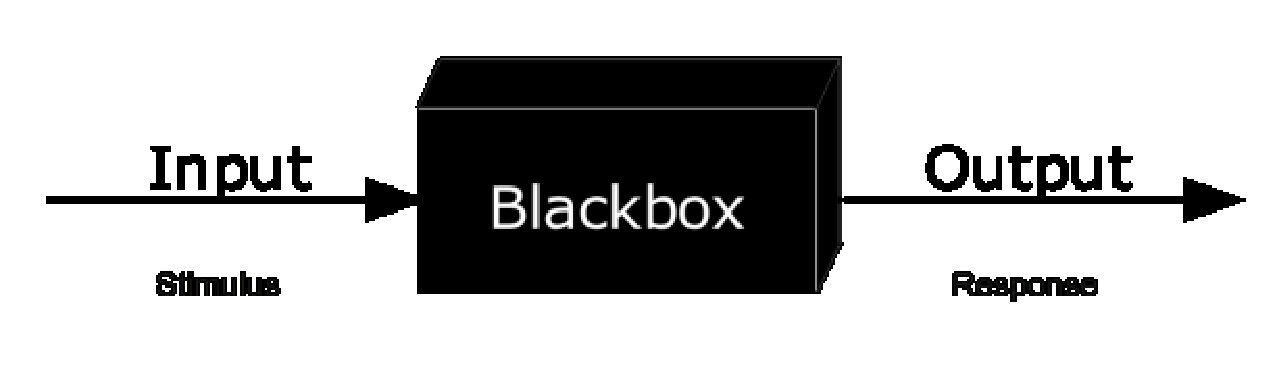
\includegraphics[width=0.8\textwidth]{blackbox.eps}
\end{comment}

\begin{frame}
\frametitle{Latency vs Throughput}
\begin{block}{Nonlinear in general}
Gradual change at low throughput, rapid increase near system capacity 
\end{block}
\begin{figure}
    \centering
    \includegraphics[scale = 0.35]{two_regions_bare.eps}
\end{figure}
\end{frame}
\begin{frame}
\frametitle{Latency vs Throughput}
\begin{block}{Focus on low-throughput region}
Linear relationship between latency and throughput
\end{block}
\begin{figure}
    \centering
    \includegraphics[scale = 0.35]{two_regions.eps}
\end{figure}
\end{frame}

\section{Model}
\begin{frame}
\frametitle{Multiple Linear Regression}
Dependent variable $y$, independent variables $x_1,\ldots,x_p$
\begin{displaymath}{
y_i = \beta_1 x_{i1}+\ldots+\beta_{p}x_{ip}+\epsilon_i
}\end{displaymath}

Do a multiple linear regression to find the coefficients $\beta_i$.  Then for a test instance $VM_{test}$ with $x_{test,i}$, find:
\begin{displaymath}{
y_{test} = \beta_1 x_{test,1}+\ldots+\beta_{p}x_{test,p}
}\end{displaymath}

\end{frame}

\begin{frame}
\frametitle{Multiple Linear Regression}
Predicted coefficient of determination:
\begin{displaymath}
R_{predicted}^2=1-\frac{\sum_{i=1}^{n} (y_{test,i} - \hat{y}(x_{test,i}))^{2}}{\sum_{i=1}^{n} (y_{test,i} - \bar{y_{test}})^{2}}
\end{displaymath}
where
\begin{displaymath}
\hat{y}(x_{test,i})=\sum_{i=1}^{n} \beta_i x_{test,i}
\qquad\text{and}\qquad
\bar{y}_{test}=\frac{1}{n}\sum_{i=1}^{n} y_{test,i}
\end{displaymath}
\end{frame}
\section{Testing}

\begin{frame}
\frametitle{Databases used in testing}
\begin{block}{Redis}
Most popular Key-value database
\end{block}
\begin{block}{Apache Cassandra}
Most scalable NoSQL database
\end{block}
\begin{block}{MySQL}
Most widely used open-source RDBMS
\end{block}
\end{frame}

\begin{frame}
\frametitle{Benchmark specifics}
\begin{enumerate}
\item Yahoo! Cloud Serving Benchmark 
\item YCSB client on m4.2xlarge EC2 instance with Ubuntu Linux 14.04
\item testing from same Amazon zone/region
\item preload database before each test
\item check client system load to make sure client is not the bottleneck
\end{enumerate}
\end{frame}

\begin{frame}
\frametitle{Benchmark specifics}
AWS instances used in testing:
\begin{table}
\begin{tabular}{|r|l|c|r|l|} \hline
Instance name & Abbr.& \# cores&Memory&Network\\ \hline
m3.large & $VM_1$ & 2 & 7.5 GB & Moderate\\ \hline
m3.xlarge & $VM_2$ & 4 & 15 GB & Moderate\\ \hline
m3.2xlarge & $VM_3$ & 8 & 30 GB & High\\ \hline
r3.large & $VM_4$ & 2 & 15 GB & Moderate\\ \hline
r3.xlarge & $VM_5$ & 4 & 30.5 GB & Moderate\\ \hline
r3.2xlarge & $VM_6$ & 8 & 61 GB & High\\ \hline
\hline\end{tabular}
\end{table}
\end{frame}

\section{Results}

\begin{frame}
\frametitle{Redis}
\begin{enumerate}
\item key/value NoSQL database
\item deployed with Amazon ElastiCache
\item only used one read replica
\end{enumerate}
\end{frame}

\begin{frame}
\frametitle{Redis}
\begin{table}
\centering
\caption{Redis Latency $R_{predicted}^2$ for $VM_2$}
\begin{tabular}{|r|r|l|} \hline
read&write&Training Set\\ \hline
-0.648416 & -1.12245  & $\{VM6\}$ \\ \hline 
0.51488 &  0.41527 & $\{VM6,VM5\}$ \\ \hline 
0.738979 &  0.738969 & $\{VM6,VM3,VM5\}$ \\ \hline 
0.776002 & 0.756578  & $\{VM6,VM3,VM5,VM4\}$ \\ \hline 
0.837957 &  0.827944 & $\{VM6,VM3,VM5,VM4,VM1\}$ \\ \hline 
\hline\end{tabular}

% \centering
% \caption{Redis $R_{predicted}^2$ for $VM_2$}
% \begin{tabular}{|r|r|l|} \hline
% reads&writes&Training Set\\ \hline
% -0.648416 & -1.12245  & VM6 \\ \hline 
% 0.51488 &  0.547705 & VM6 VM5 \\ \hline 
% 0.738979 & 0.738969  & VM6 VM5 VM3 \\ \hline 
% 0.832156 &  0.756578 & VM6 VM5 VM3 VM1 \\ \hline 
% 0.837957 & 0.827944  & VM6 VM5 VM3 VM1 VM4 \\ \hline 
% \hline\end{tabular}
%\end{minipage}
% \begin{minipage}[b]{0.25\linewidth}
% \centering
% \caption{Redis $R_{predicted}^2$ for $VM_2$}
% \begin{tabular}{|r|r|l|} \hline
% reads&writes&Training Set\\ \hline
% -0.559516 & -0.47657  & VM5 \\ \hline 
% 0.260701 &  0.29636 & VM5 VM3 \\ \hline 
% 0.738979 &  0.738969 & VM5 VM3 VM6 \\ \hline 
% 0.776002 & 0.756578  & VM5 VM3 VM6 VM4 \\ \hline 
% 0.837957 & 0.827944  & VM5 VM3 VM6 VM4 VM1 \\ \hline 
% \hline\end{tabular}

% \centering
% \caption{Redis $R_{predicted}^2$ for $VM_2$}
% \begin{tabular}{|r|r|l|} \hline
% reads&writes&Training Set\\ \hline
% -0.559516 & -0.47657  & VM5 \\ \hline 
% 0.51488 & 0.547705  & VM5 VM6 \\ \hline 
% 0.738979 & 0.738969  & VM5 VM6 VM3 \\ \hline 
% 0.776002 & 0.756578  & VM5 VM6 VM3 VM4 \\ \hline 
% 0.837957 & 0.827944  & VM5 VM6 VM3 VM4 VM1 \\ \hline 
% \hline\end{tabular}
% \end{minipage}
\end{table}
\end{frame}

\begin{frame}
\frametitle{Redis}
  \begin{figure}
    \centering
    \includegraphics[scale = 0.4]{bar_read_avg_latency.eps}
  \end{figure}
\end{frame}

\begin{frame}
\frametitle{Redis}
  \begin{figure}
    \centering
    \includegraphics[scale = 0.4]{bar_write_avg_latency.eps}
  \end{figure}
\end{frame}

\begin{frame}
\frametitle{Redis}
\begin{figure}
\begin{tabular}{cc}
 \includegraphics[width=0.35\textwidth]{fit_write_avg_latency_r3_2x_m3_2x_r3_x_r3__m3__m3_x.eps} &
\includegraphics[width=0.35\textwidth]{fit_write_avg_latency_r3_2x_r3_x_m3_2x_m3__r3__m3_x.eps} \\
\includegraphics[width=0.35\textwidth]{fit_write_avg_latency_r3_x_m3_2x_r3_2x_r3__m3__m3_x.eps} &
\includegraphics[width=0.35\textwidth]{fit_write_avg_latency_r3_x_r3_2x_m3_2x_r3__m3__m3_x.eps} \\ 
\end{tabular}
\caption{Prediction of Redis write latency on $VM_2$ compared for model calibration using a variety of training sets ranging in size from 1 to 5 VM types.}
\end{figure}
\end{frame}

\begin{frame}
\frametitle{Apache Cassandra: Table/Key-Value hybrid NoSQL database}
\begin{enumerate}
\item high availability provided by replication
\item Cassandra prioritizes availability and performance over consistency \begin{figure}[htbp]
\centering
\includegraphics[width=0.4\textwidth]{CAP_diagram.pdf}
\end{figure}
\end{enumerate}
\end{frame}

\begin{frame}
\frametitle{Apache Cassandra: Table/Key-Value hybrid NoSQL database}
\begin{enumerate}
\item Cassandra clusters with 5 nodes
\item replication factor of three
\item consistency level of ONE (weak/eventual consistency)
\end{enumerate}
\end{frame}

\begin{frame}
\frametitle{Apache Cassandra}
  \begin{figure}
    \centering
    \includegraphics[scale = 0.4]{cassandra_bar_read_avg_latency.eps}
  \end{figure}
\end{frame}

\begin{frame}
\frametitle{Apache Cassandra}
  \begin{figure}
    \centering
    \includegraphics[scale = 0.4]{cassandra_bar_write_avg_latency.eps}
  \end{figure}
\end{frame}

\begin{frame}
\frametitle{Apache Cassandra}
\begin{figure}
\includegraphics[width=0.25\textwidth]{cassandra_fit_read_avg_latency_m3_2x_m3__r3_2x_m3_x_r3_x_r3_.eps}
\includegraphics[width=0.25\textwidth]{cassandra_fit_read_avg_latency_m3_2x_m3__r3_2x_r3_x_m3_x_r3_.eps}
\includegraphics[width=0.25\textwidth]{cassandra_fit_read_avg_latency_r3_x_m3__r3_2x_m3_2x_m3_x_r3_.eps}
\includegraphics[width=0.25\textwidth]{cassandra_fit_read_avg_latency_r3_x_r3_2x_m3__m3_2x_m3_x_r3_.eps}
\caption{Prediction of Cassandra read latency on $VM_4$ compared for model calibration using a variety of training sets ranging in size from 1 to 5 VM types.}
\end{figure}
\end{frame}

\begin{frame}
\frametitle{Apache Cassandra}
\begin{figure}
\includegraphics[width=0.25\textwidth]{cassandra_fit_write_avg_latency_m3_2x_m3__r3_2x_m3_x_r3_x_r3_.eps}
\includegraphics[width=0.25\textwidth]{cassandra_fit_write_avg_latency_m3_2x_m3__r3_2x_r3_x_m3_x_r3_.eps}
\includegraphics[width=0.25\textwidth]{cassandra_fit_write_avg_latency_m3_x_m3_2x_r3_2x_m3__r3_x_r3_.eps}
\includegraphics[width=0.25\textwidth]{cassandra_fit_write_avg_latency_m3_x_m3_2x_r3_2x_r3_x_m3__r3_.eps}
\caption{Prediction of Cassandra write latency on $VM_4$ compared for model calibration using a variety of training sets ranging in size from 1 to 5 VM types.}
\end{figure}
\end{frame}

\begin{frame}
\frametitle{Redis}
\begin{enumerate}
\item RDBMS database
\item deployed with Amazon RDS
\end{enumerate}
\end{frame}

\begin{frame}
\frametitle{MySQL}
  \begin{figure}
    \centering
    \includegraphics[scale = 0.3]{mysql_fit_read_avg_latency.eps}
    \caption{Read latency/throughput plot for MySQL. Although our multiple linear regression model offers a poorer prediction for MySQL than for our other case studies, we continue to observe an improvement in its efficacy upon increasing the diversity of the training set. }
    \label{figure:mysql}
  \end{figure}
\end{frame}

\section{Conclusions}

\begin{frame}
\frametitle{Conclusions}
\begin{block}{Diversity of VM instance types}
Opportunity for data modeling
\end{block}
\begin{block}{Tested Latency vs. Throughput for 3 common database applications}
Redis, Cassandra, MySQL
\end{block}
\begin{block}{Found Model Accuracy improved with larger training sets}
With larger dataset, possibility of more accurately predicting performance for new VM instance types
\end{block}
\end{frame}

%------------------------------------------------
\begin{comment}
\begin{frame}
\frametitle{Bullet Points}
\begin{itemize}
\item Lorem ipsum dolor sit amet, consectetur adipiscing elit
\item Aliquam blandit faucibus nisi, sit amet dapibus enim tempus eu
\item Nulla commodo, erat quis gravida posuere, elit lacus lobortis est, quis porttitor odio mauris at libero
\item Nam cursus est eget velit posuere pellentesque
\item Vestibulum faucibus velit a augue condimentum quis convallis nulla gravida
\end{itemize}
\end{frame}

%------------------------------------------------

\begin{frame}
\frametitle{Blocks of Highlighted Text}
\begin{block}{Block 1}
Lorem ipsum dolor sit amet, consectetur adipiscing elit. Integer lectus nisl, ultricies in feugiat rutrum, porttitor sit amet augue. Aliquam ut tortor mauris. Sed volutpat ante purus, quis accumsan dolor.
\end{block}

\begin{block}{Block 2}
Pellentesque sed tellus purus. Class aptent taciti sociosqu ad litora torquent per conubia nostra, per inceptos himenaeos. Vestibulum quis magna at risus dictum tempor eu vitae velit.
\end{block}

\begin{block}{Block 3}
Suspendisse tincidunt sagittis gravida. Curabitur condimentum, enim sed venenatis rutrum, ipsum neque consectetur orci, sed blandit justo nisi ac lacus.
\end{block}
\end{frame}

%------------------------------------------------

\begin{frame}
\frametitle{Multiple Columns}
\begin{columns}[c] % The "c" option specifies centered vertical alignment while the "t" option is used for top vertical alignment

\column{.45\textwidth} % Left column and width
\textbf{Heading}
\begin{enumerate}
\item Statement
\item Explanation
\item Example
\end{enumerate}

\column{.5\textwidth} % Right column and width
Lorem ipsum dolor sit amet, consectetur adipiscing elit. Integer lectus nisl, ultricies in feugiat rutrum, porttitor sit amet augue. Aliquam ut tortor mauris. Sed volutpat ante purus, quis accumsan dolor.

\end{columns}
\end{frame}

%------------------------------------------------
%\section{Second Section}
%------------------------------------------------

\begin{frame}
\frametitle{Table}
\begin{table}
\begin{tabular}{l l l}
\toprule
\textbf{Treatments} & \textbf{Response 1} & \textbf{Response 2}\\
\midrule
Treatment 1 & 0.0003262 & 0.562 \\
Treatment 2 & 0.0015681 & 0.910 \\
Treatment 3 & 0.0009271 & 0.296 \\
\bottomrule
\end{tabular}
\caption{Table caption}
\end{table}
\end{frame}

%------------------------------------------------

\begin{frame}
\frametitle{Theorem}
\begin{theorem}[Mass--energy equivalence]
$E = mc^2$
\end{theorem}
\end{frame}

%------------------------------------------------

\begin{frame}[fragile] % Need to use the fragile option when verbatim is used in the slide
\frametitle{Verbatim}
\begin{example}[Theorem Slide Code]
\begin{verbatim}
\begin{frame}
\frametitle{Theorem}
\begin{theorem}[Mass--energy equivalence]
$E = mc^2$
\end{theorem}
\end{frame}\end{verbatim}
\end{example}
\end{frame}

%------------------------------------------------

\begin{frame}
\frametitle{Figure}
Uncomment the code on this slide to include your own image from the same directory as the template .TeX file.
%\begin{figure}
%\includegraphics[width=0.8\linewidth]{test}
%\end{figure}
\end{frame}

%------------------------------------------------

\begin{frame}[fragile] % Need to use the fragile option when verbatim is used in the slide
\frametitle{Citation}
An example of the \verb|\cite| command to cite within the presentation:\\~

This statement requires citation \cite{p1}.
\end{frame}

%------------------------------------------------

\begin{frame}
\frametitle{References}
\footnotesize{
\begin{thebibliography}{99} % Beamer does not support BibTeX so references must be inserted manually as below
\bibitem[Smith, 2012]{p1} John Smith (2012)
\newblock Title of the publication
\newblock \emph{Journal Name} 12(3), 45 -- 678.
\end{thebibliography}
}
\end{frame}
\end{comment}

%------------------------------------------------

\begin{frame}
\Huge{\centerline{The End}}
\end{frame}

%----------------------------------------------------------------------------------------
\end{document}
\documentclass[a4paper,11pt]{article}
\usepackage{color}
\usepackage{comment}
\usepackage{url}
\usepackage{doublefig}
\usepackage{float}
\usepackage{graphicx}
\usepackage{amsmath}
\usepackage{amsthm}
\usepackage{enumitem}
%\usepackage{refcheck}
\usepackage[caption = false]{subfig}
%\usepackage[demo]{graphicx}

%\pagenumbering{arabic}

\begin{document}
%\nocite{*}
\title{Towards Performance Modeling as a Service by Exploiting Resource Diversity in the Public Cloud}

\author{
Mark Meredith\\
       Dept. of Comp. Sci. and Eng.\\
       The Penn State University\\
       University Park, PA 16802\\
       mwm126@cse.psu.edu
}
\maketitle
%\setcounter{1}
\pagenumbering{arabic}

\begin{abstract}
%One of the main benefits of virtualization through cloud computing is the ready availability of large rapid virtual machines for rapid application deployment. As computing hardware advances, cloud computing vendors offer new virtual machines with new performance characteristics, adding to the large set of virtual machine types to choose from. Many virtual machine types are available, with varying performance and pricing options. In this work we present a statistical model for estimating the performance of new virtual machine types based on knowledge of existing types. This model is based on data collected by running the Yahoo! Cloud Services Benchmark (YCSB). The databases surveyed are the key-value database Redis, deployed on Amazon Elasticache, and the NoSQL databases Apache Cassandra, deployed on Amazon Elastic Compute Cloud. We tested these on a variety of Amazon virtual machines types.

%A key difference between 
Cloud computing platforms such as Amazon EC2, Google Computing Engine, and Microsoft Azure
offer dozens of virtual machine (VM) types with a wide range of resource capacity vs. price trade-offs, requiring a customer to consider numerous resource configurations when evaluating service needs. This report investigates the possibility of using the diversity of VM types to predict the performance of new VM types using black box modeling. The performance model used is a multiple linear regression of the average server response time, server load (throughput in requests per second), the number of CPU cores, and the memory in the procured VM. For three commonly used database servers - Redis (key-value stores), Apache Cassandra (NoSQL) and MySQL -  the model accuracy increases for larger sets of VMs.  E.g., for Redis, the $R^2_{predicted}$ measure of model efficacy improves from 0.4-0.5 with 2 VM types for training and 0.7 for 3 VM types to 0.8 for 4 VM types.  These results suggest further interesting research challenges, such as the possibility of automating the process of calibrating performance models using diverse resource types on a public cloud leading to ``performance modeling as a service.''

\end{abstract}

\section{Introduction}
\vspace{10pt}

%Cloud vendors offer a lot of different virtual machine instance types. Cloud tenants needs to determine what benefit new virtual machine types will bring to their applications.


Many enterprises are migrating their information technology (IT) needs to public cloud computing platforms, a trend that is projected to continue unabated in the foreseeable future~\cite{forbes}. Among the most important reasons behind these ``tenants'' choosing to procure their IT needs from a public cloud is the promise of lower costs. To effectively realize these cost-related benefits, however, it is crucial that these tenants carry out careful dynamic procurement of IT resources to match their evolving needs. Numerous studies show that approaches based on over-provisioning or other ``crude'' estimates of resource needs may negate the cost benefit potential that migrating to a public cloud may offer~\cite{takmig,xxx}. Therefore, tenant-side resource procurement has emerged as an area of active research with different aspects of it receiving attention both in academic papers~\cite{xxx} and industrial products~\cite{xxx}. 

Procuring resources cost-effectively from a public cloud provider poses significant technical challenges. One such challenge concerns the problem of determining the set of IT resources (including their capacities) - virtual machines, the virtual network connecting these VMs, storage, etc. - that would be needed to cost-effectively meet the predicted workload of the tenant's software application while offering satisfactory performance and availability to its users. In order to solve this problem, a tenant must first solve the problem of assessing the performance the users of its application software are likely to experience if the application were assigned a given set of IT resources to meet its predicted workload. Our interest in this paper is in this latter problem, often labeled {\it application performance modeling}~\cite{sigmetrics05,chrisstewart-eurosys,anshul,bianca,gosiaasser,lucy-cherkasova}. 

%\noindent{\bf The Problem:} **state the problem.** 

% explain why it is challenging to solve this problem in a public cloud ecosystem
Whereas application performance modeling has been an area of extensive research for many decades across many communities, solving it for the public cloud ecosystem presents a tenant with non-trivial novel sources of complexity. In particular, most modeling solutions have traditionally been developed for settings involving privately owned and operated data centers or clusters. These solutions may not be readily adapted to a public cloud. %A typical example of such a private setting is a data center or a cluster privately owned and operated by an enterprise that is considering replacing it in favor of a move of its IT needs to a public cloud. 

\begin{figure}[htbp]
\centering
\includegraphics[width=0.45\textwidth]{cloud_vm_types.eps}
\caption{An illustration of the diversity in VM capacities offered by popular public cloud providers. We show VMs with a wide range of CPU and memory capacities offered by Amazon EC2~\cite{amazon-ec2}, Google Compute Engine~\cite{google-computeengine}, and Microsoft Azure~\cite{windows-azure}.} \label{fig:diversity}
%\vspace{-10pt}
\end{figure}


Arguably, the most important difference between  these two settings (from the point of view of application performance modeling) is the immense {\it diversity of resources} that a typical public cloud offers.~\footnote{There are other important differences complementary to our focus in this paper and part of our future work. E.g., in a private setting, the user of a machine (tenant application) coincides with its owner while in a public setting the two are separated via virtualization techniques with implications for how much information about physical resource usage is available to the tenant's models. } We will focus on virtual machines (VMs) as the resource type of interest in this work although our arguments likely apply to other resource types as well. To appreciate this diversity, let us consider some examples from the most prominent public cloud providers that offer many VM types since they need to cater to many different types of customers.  ~\mm{Here virtual machine instance types are organized in groups based on use case.  Instances within a group generally have the same CPU generation and clock speed, and vary by the number of CPUs and memory.  Amazon EC2 offers over 40 VM types organized in eight different groups, varying in CPU, memory, network bandwidth, storage speed, and pricing~\cite{amazon-ec2}. Google Compute Engine offers 15 instance types organized in four groups: Standard, High CPU, High Memory, and Shared Core (for lightweight applications)~\cite{google-computeengine}. Finally, Windows Azure ...~\cite{windows-azure}. Figure~\ref{figure:diversity} shows 30 VM instance types organized into four groups: Basic, Standard, Optimized, and Optimized (version 2). ...} 

A typical privately owned data center, on the other hand, is likely to possess a much smaller number of machine types. Keeping machines (and their software configurations) relatively homogeneous brings about significant benefits related to ease of system administration and cost savings (e.g., due to bulk purchase offers from IT vendors). Although factors such as incremental procurement over time, meeting specialized needs (e.g., machines with GPUs), etc.,  do result in some differences among machine types even in a private data center, the overall degree of heterogeneity is significantly smaller than that seen in a  public cloud.

 

This high diversity of resource types in a public cloud introduces an additional source of complexity into a tenant's decision-making. Since the number of resource types in traditional IT environments are small and relatively fixed, performance models have conventionally been developed and calibrated using performance measurements (``profiling'') on the same/similar type of machines on which the application would eventually execute. On the other hand, a tenant of a public cloud would be interested in being able to predict the performance that its workload might experience on a wide variety of resource types that the provider offers. This is because which resource types are the most cost-effective for a tenant's workload might change over time due to: (i) changes in the tenant's own workload (e.g., many applications show periodic time-of-day or seasonal variations in their workload intensities) and (ii) dynamism and variety in the cloud provider's pricing schemes (e.g., Amazon EC2 offers spot pricing for most of its instance types and such spot instances are usually much cheaper than their on-demand counterparts). Clearly, approaches based on calibrating a tenant's performance models separately on the dozens of resource types that public clouds offer are likely to not be scalable. Additionally, such approaches may prove to be expensive. 

% introduce the idea of exploiting diversity instead of letting it be a hindrance. 
We wish to explore if a tenant might actually be able to benefit from this diversity by deliberately and carefully exploiting it to ease the creation and calibration of effective performance models. *** explain why we expect this to be the case. *** This leads us to explore the following hypothesis: {\it diversity of VMs in a public cloud can aid in the calibration of tenant application performance models on unseen VMs.} 

An important aspect of our hypothesis worth highlighting is that it is not tied to a specific performance modeling approach. ** expand this **

\noindent {\bf Our Approach and Contributions:} In this paper, we take a small first step towards exploring the above idea. Specifically, we devise a multi-linear regression modeling framework for predicting the performance of interactive data storage server applications. We calibrate this model for three different types of real-world applications: (i) Redis, a ..., (ii) Apache Cassandra, a ..., (iii) Mysql, a popular open-source ACID database. We ... 

Our key findings are as follows:
\begin{itemize}
\item ...
\item ...
\item ...
\end{itemize}


To the best of our knowledge, ... On the one hand, our work is highly complementary to traditional performance modeling research. At the same time, it opens up a promising new area for further research. As part of our own future work, we plan to ... ** discuss the possibility of offering PMaaS as a key implication of our work as well as being an interesting direction for future research. **

The rest of this paper is organized as follows. In Section~\ref{sec:back}, we provide an overview of a generic cost-conscious tenant's decision-making and where application performance modeling fits within it.  In Section~\ref{sec:model}, we describe the performance modeling techniques that we employ.  In Section~\ref{sec:eval}, we present our empirical evaluation of our hypothesis using three real-world applications as our case studies. We discuss related work in Section~\ref{sec:related}.  Finally, we discuss unresolved challenges and future directions in Section~\ref{sec:future} and conclude in Section~\ref{sec:conclus}. 
 

%Solution: test your application on different VM types and find out?

%present the problem, its significance, and key challenges
 
%explain why the state-of-the-art may not be adequate, particularly as clouds move towards higher levels of utilization and dynamism

%explain our key ideas and contributions

%\section{Context and Overview}
\label{sec:back}
\vspace{10pt}

%big picture overview of tenant-side decision-making, where PMaaS fits within this, mention the specific assumptions we make, the chosen environment, which ideas are likely to generalize to other settings
 
\begin{figure*}%[htbp]
\centering
\includegraphics[width=0.8\textwidth]{system}
\caption{An overview of interactions between the performance modeling problem we study and other aspects of the overall decision-making for a cost-conscious tenant procuring resources from a public cloud. }
\label{fig:diagram}
%\vspace{-10pt}
\end{figure*}

Figure~\ref{fig:diagram} shows the essential elements making up the decision-making that a general cost-conscious tenant might carry out when procuring resources from a public cloud. In particular, it clarifies the role of application performance modeling within this overall decision-making and its interaction with other elements. 
%** expand this, 
The tenant would employ observations of its workload intensity in the past to predict its future workload. Consider the example of a key-value store or a database application that we employ in our evaluation in Section~\ref{sec:eval}. Such an application might keept track of request arrival rates (possibly for different request classes) and then use a suitable prediction mechanism for estimating future arrival rate. Whereas some tenant applications exhibit significant predictability (e.g., captured well via Markovian or autoregressive models)~\cite{xxx}, others are known to exhibit poor predictability and must resort to short-term (``myopic'') estimates~\cite{xxx}. Regardless, having made these predictions, the tenant must then ascertain the number and type of VMs that it must procure from the cloud to meet its performance needs (or deallocate from its existing resource pool). 

%Figure~\ref{fig:diagram} shows 
We show one way of thinking about this decision-making~\footnote{The actual realization of this overall decision-making may be different from how we describe it here. Our description is deliberately designed to highlight the role of the application performance model.}, wherein the tenant determines (using its application performance model) multiple VM allocation choices that would allow it to meet its predicted workload with the requisite performance goals. These choices are then compared in terms of their costs (or expected profits, if the tenant wishes to maximize expected profits rather than minimizing costs) via an optimization problem that incororates idiosyncrasies of the prices offered by the public cloud. Finally, the most cost-effective choice identified by the optimizer is used as the basis for actually procuring the appropriate number and type of VMs from the cloud provider. 

%**point to related work, repeat that our arguments are not tied to a particular modeling technique. **
Significant research exists both on predicting workloads and on performance modeling (see Section~\ref{sec:related}) for a wide variety of application types. Recall that our interest in this paper is not on devising new techniques for workload prediction or application performance modeling. Rather, we are interested in evaluating the role VM diversity might play in calibrating a {\it given} performance model. Towards this, we next describe one popularly used modeling approach that we adapt for our purposes. 

%what about the costs of PMaaS itself? how to make it practical? might providers actually offer it as a service?

\section{Our Modeling Methodology}
\label{sec:model}
\vspace{10pt}

This section describes the general performance modeling ideas used. In Section~\ref{sec:eval}, %we describe how 
this basic model is adapted to three application case studies on the Amazon AWS cloud. The primary interest in this paper is not in identifying the most accurate performance model but rather in exploring if diversity in the VMs used for calibrating the chosen model helps improve its efficacy. 
Therefore, although numerous modeling choices exist in the literature for such applications, we use a relatively simple multiple linear regression approach because: (i) it serves as a good starting point for evaluating the hypothesis, (ii) it is easy to cast, train, and evaluate, and (ii)it  works well - especially under low/moderate throughputs for the normal operating regions of well-provisioned, performance-sensitive tenant workloads.

%\subsection{Background on Multiple Linear Regression}
\noindent{\bf Multiple Linear Regression:} Given a data set \\ $\{y_i,x_{i1},\ldots,x_{ip}\}^n_{i=1}$, a linear regression on multiple independent variables $x_{p}$ and dependent variable $y$ is a set of parameters $\beta_i$ that model a linear relationship between $y$ and $x_{i}$~\cite{CMUStatsBook}.

\begin{displaymath}{
y_i = \beta_1 x_{i1}+\ldots+\beta_{p}x_{ip}+\epsilon_i
}\end{displaymath}

The parameters $\epsilon_i$ are the error terms, an unobserved random variable.  The parameters $\beta_i$ are chosen to minimize the values of $\epsilon_i$ for the entire data set.  Specifically, the $\beta_i$ are chosen to minimize the sum of squares $\sum_{i=1}^{n} \epsilon^2_i$.

%\subsection{Model}
%Our goal is to model the performance of different virtual machine instance types, and show a correlation between the performance of those applications that can be used to predict the performance of those applications on new virtual machine instance types.

%The performance of a server application is evaluated as the time latency $y_{L}$ for responding to a request.  
We choose as our dependent variable the average latency $y_{L}$ and as our independent variables: (i) workload/application properties - throughput, degree of replication, and read/write ratio and (ii) resource capacity of the VMs being used - number of CPU cores, clock rate of each CPU, memory, network bandwidth, and type of storage (SSD vs. magnetic). 
%is the dependent variable in our model.  The benchmarks are run at multiple levels of throughput (requests/second), which is taken as an independent variable $x_{T}$

%Virtual machine instances vary by in many ways:  the type of CPU, CPU clock speed, number of CPUs, amount of memory, type or storage (SSD vs magnetic), amount of storage, and available network bandwidth.  Each of these parameters can be modeled by as an independent variable $x_p$.

We define a training set $S = \{VM_i\}^n_{i=1}$ as a set of virtual machines, each characterized by $x_p$.  In each of our experiments, we run the application whose performance we wish to model on  $VM_i$ for various $x_{T}$ and measure the latency $x_{L}$.  We then find a multiple linear regression $M_S$ on $\{y_{iL},x_{iT},\ldots,x_{ip}\}^n_{i=1}$.  (For a given instance $VM_i$, the values of $x_{ip}$ are fixed for all measurements for that instance.) 

%We then consider another instance $VM_{test}\notin S$ and use $M_S$ to predict the dependent variable $y_L$.

\begin{figure}
    \centering
    \includegraphics[scale = 0.35]{two_regions.eps}
    \caption{Two regions of latency vs. throughput for Redis. }
    \label{figure:combined}
\end{figure}

\noindent{\bf Measure of Model Efficacy:} We use the predicted coefficient of multiple determination ($R^2_{predicted}$) as our measure of model accuracy which is defined as: 
\theoremstyle{definition}
\newtheorem{mydef}{Definition}
\begin{mydef}
For a test instance $VM_{test}$ with $x_{test,i}$,
\begin{displaymath}
R_{predicted}^2=1-\frac{\sum_{i=1}^{n} (y_{test,i} - \hat{y}(x_{test,i}))^{2}}{\sum_{i=1}^{n} (y_{test,i} - \bar{y_{test}})^{2}}
\end{displaymath}
where
\begin{displaymath}
\hat{y}(x_{test,i})=\sum_{i=1}^{n} \beta_i x_{test,i}
\end{displaymath}
and $\bar{y}_{test}$ is the mean of $y_{test,i}$.
\end{mydef}

%\subsubsection{Input and Predicted Variables}

To see evidence supporting our hypothesis, we expect to see the following behavior: for larger training sets $S$, the model should fit better to $VM_{test}$, corresponding to an increasing $R^2_{predicted}$, assuming sufficient variability in the values of $x_p$ for $VM_j\in S$ to cover the values of $x_p$ for $VM_{test}$.  

\noindent{\bf Discussion:} Our linear regression based model is known to perform poorly when queueing delays become dominant contributors to overall latency~\cite{Stewart07}. 
For example, if we were to model the entire set of latency observations (for experiements done using Redis, more details
in Section~\ref{sec:redis}) using our model, we would obtain a poorer predictor than the two separate linear regression
models shown in Figure~\ref{figure:combined}, one each for the ``low/moderate'' (Region 1) and ``high'' (Region 2) throughput regions. This suggests two points: (i) using domain knowledge (e.g., the distinction between low and high throughput regions), a 
tenant may be able to use linear regression to obtain better models, and (ii) more sophisticated models may be 
warranted for the needs of certain tenants. Again, since our interest is in the impact of diversity on modeling accuracy,
we focus only on modeling performance in Region 1 for the rest of this paper. 

It is important to keep in mind the basic assumption of linear regression about the independent variables being independent of each other (i.e., the $x_p$ for $VM_j\in S$ need to be independent). Interestingly, among the independent
variables in our model, the number of cores and memory capacity are prone to be problematic on this front - typically
larger VMs come both with more CPUs and more memory - see Figure~\ref{fig:diversity}. To overcome this problem, we attempt to choose VM types
in our experiments where this correlation is weak. Furthermore, the results we present in this paper are for a subset
of our experimental findings wherein the entire working set fits in VM memory, rendering memory moot as a predictor of
performance (we do incorporate memory in our more general experiments). Finally, the potential shortcomings of predicted 
$R^2$ as a measure of model accuracy should be kept in mind when interpreting our results~\cite{CMUStatsBook}. 
%}
  
%\subsubsection{Measure of Model Efficacy}  
  
%\subsection{Discussion}
%\vspace{10pt}


\section{Evaluation}
\label{sec:eval}
\vspace{10pt}

\begin{comment}
~\bu{Suggestions for creating a first draft:
\begin{itemize}
\item In Section 4.1: When describing our experimental setup, refer to Table 1 to say we restrict our attention to these 6 VMs from AWS and only use num cores, memory, num replicas, and throughput as our independent variables. Our dependent variables are average read and write latencies.
\item Have a generic figure showing a YCSB client and one of our case studies with 3 replicas. 
\item For Sections 4.2-4.4, describe the graphs/tables being presented in some detail, identify any trends. Conclude each with a list of "Key insights"
\item Most figures and tables need more clarity on what exactly was the training set, for which VM the prediction is being done, etc. All figures need larger fonts on their axes, labels, etc. 
\item Replace R-squared with $R^2_{predicted}$. 
\end{itemize}

\end{comment}

\subsection{Methodology and Setup}
\vspace{10pt}

\begin{table}
\centering

\begin{tabular}{|r|l|c|r|l|} \hline
Instance name & Abbr.& \# cores&Memory&Network\\ \hline
m3.large & $VM_1$ & 2 & 7.5 GB & Moderate\\ \hline
m3.xlarge & $VM_2$ & 4 & 15 GB & Moderate\\ \hline
m3.2xlarge & $VM_3$ & 8 & 30 GB & High\\ \hline
r3.large & $VM_4$ & 2 & 15 GB & Moderate\\ \hline
r3.xlarge & $VM_5$ & 4 & 30.5 GB & Moderate\\ \hline
r3.2xlarge & $VM_6$ & 8 & 61 GB & High\\ \hline
\hline\end{tabular}
\caption{AWS instance types employed in our evaluation. }
\label{table:awstypes}
\end{table}

We carry out our evaluation on the EC2 public cloud offered by Amazon Web Services (AWS)~\cite{amazon-ec2}. We adapt our generic performance model from Section~\ref{sec:model} for three different types of latency-sensitive data-serving applications: (i) Redis (an in-memory open-source NoSQL key-value store)~\cite{redis}, (ii) Apache Cassandra (a NoSQL key-value store that can be configured for different consistency levels), and the popular MySQL ACID database~\cite{mysql}. We use the open-source Yahoo! Cloud Serving Benchmark (YCSB) as our workload generator~\cite{Cooper:2010:BCS:1807128.1807152}. We run the YCSB client on a m4.2xlarge EC2 instance running Ubuntu Linux 14.04. We monitor the system load average on the client machine to verify that the client is not the bottleneck during our tests.


  \begin{figure*}
    \centering
    \includegraphics[scale = 0.4]{bar_read_avg_latency.eps}
    \includegraphics[scale = 0.4]{bar_write_avg_latency.eps}
    \caption{\textbf{Redis read and write $R^2_{predicted}$ vs training set.  We find that $R^2_{predicted}$ improves consistency with more diverse training sets for a wide range of training set choices supporting our basic hypothesis.}}
    \label{figure:redisbarreadwrite}
  \end{figure*}



We describe a subset of our overall results wherein for each experiment %case 
we load the concerned database with 1,000,000 records, each containing ten fields of 100 bytes each (the default). This amounts to an overall working set of about 1GB. Each experiment consists of subjecting the database to a particular thoughput and recording the average latency (separately for reads and writes). YCSB defines several standard workloads that we experiment with. We experiment with different workloads offered by YCSB and present a subset of our overall results - workload ``A'' for MySQL and ``B'' for Redis and Cassandra. Workload A has 50\% read and 50\% write requests and employs a uniform popularity distribution. Workload B has 95\% reads and 5\% writes, and  the popularity of requests is chosen based on a zipfian distribution. We repeat each experiment several times to achieve significantly tight confidence intervals. 
%Modeling and testing was done twice for each case study:  once for read latency and once for write latency.  The ratio of the number of write operations to read operations is another potential independent variable.  For our study, this was fixed as all testing was done with 95\%/5\% read/write.
%  Three test runs were done for each throughput and instance type to check the reproducibility of results.
Amazon EC2 is hosted in multiple geographic regions around the world, and multiple zones within each region.  We create our testing client and servers within the same region (us-west) and availability zone (2b) to minimize the effect of network latency. Finally, we pick all VMs having individual CPUs offering the same clock rate. 

 %To ensure that CPU count and memory can be safely considered independent variables (an important assumption of linear regression, recall from Section~\ref{sec:model}), 
We select the VM instances listed in Table~\ref{table:awstypes}.  
There are three instances from the M3 group (standard) and three from the R3 group (memory optimized).  The memory/CPU ratio is the same within each group, with the R3 group having twice the memory/cpu as the M3 group.  A more extensive study with more instances would allow the use of more independent variables in the model, e.g., including testing of instances in the C3 group (compute optimized), which have half as much memory/CPU as M3.

With the above choices, the measurements and modeling reported here effectively only employ a subset of all the independent variables listed in Section~\ref{sec:model}: number of CPU cores, throughput, number of replicas, and read-write ratio. In particular, our working set of 1GB fits fully within any of the chosen VMs, effectively rendering memory capacity moot as a predictive variable. In our more general experiments, however, we explore a much larger set of workload choices. 

\begin{figure*}
\subfloat[]{\includegraphics[width=0.5\textwidth]{fit_read_avg_latency_r3_2x_r3_x_m3_2x_m3__r3__m3_x.eps}} 
\subfloat[]{\includegraphics[width=0.5\textwidth]{fit_read_avg_latency_r3_2x_r3_x_m3_2x_r3__m3__m3_x.eps}}\\
\subfloat[]{\includegraphics[width=0.5\textwidth]{fit_read_avg_latency_r3_x_m3_2x_r3__m3__r3_2x_m3_x.eps}}
\subfloat[]{\includegraphics[width=0.5\textwidth]{fit_read_avg_latency_r3_x_r3_2x_m3_2x_r3__m3__m3_x.eps}} 
\caption{Prediction of Redis read latency on $VM_2$ compared for model calibration using a variety of training sets ranging in size from 1 to 5 VM types. }
\label{figure:redisfitread}
\end{figure*}

\begin{table}
\centering
\caption{Redis $R_{predicted}^2$ for $VM_2$}
\begin{tabular}{|r|r|l|} \hline
reads&writes&Training Set\\ \hline
-0.648416 & -1.12245  & VM6 \\ \hline 
0.51488 &  0.41527 & VM6 VM5 \\ \hline 
0.738979 &  0.738969 & VM6 VM3 VM5 \\ \hline 
0.776002 & 0.756578  & VM6 VM3 VM5 VM4 \\ \hline 
0.837957 &  0.827944 & VM6 VM3 VM5 VM4 VM1 \\ \hline 
\hline\end{tabular}
\label{table:redis1}
% \end{table}

% \begin{table}
\centering
\caption{Redis $R_{predicted}^2$ for $VM_2$}
\begin{tabular}{|r|r|l|} \hline
reads&writes&Training Set\\ \hline
-0.648416 & -1.12245  & VM6 \\ \hline 
0.51488 &  0.547705 & VM6 VM5 \\ \hline 
0.738979 & 0.738969  & VM6 VM5 VM3 \\ \hline 
0.832156 &  0.756578 & VM6 VM5 VM3 VM1 \\ \hline 
0.837957 & 0.827944  & VM6 VM5 VM3 VM1 VM4 \\ \hline 
\hline\end{tabular}
\label{table:redis2}
% \end{table}

% \begin{table}
\centering
\caption{Redis $R_{predicted}^2$ for $VM_2$}
\begin{tabular}{|r|r|l|} \hline
reads&writes&Training Set\\ \hline
-0.559516 & -0.47657  & VM5 \\ \hline 
0.260701 &  0.29636 & VM5 VM3 \\ \hline 
0.738979 &  0.738969 & VM5 VM3 VM6 \\ \hline 
0.776002 & 0.756578  & VM5 VM3 VM6 VM4 \\ \hline 
0.837957 & 0.827944  & VM5 VM3 VM6 VM4 VM1 \\ \hline 
\hline\end{tabular}
\label{table:redis3}
% \end{table}

% \begin{table}
\centering
\caption{Redis $R_{predicted}^2$ for $VM_2$}
\begin{tabular}{|r|r|l|} \hline
reads&writes&Training Set\\ \hline
-0.559516 & -0.47657  & VM5 \\ \hline 
0.51488 & 0.547705  & VM5 VM6 \\ \hline 
0.738979 & 0.738969  & VM5 VM6 VM3 \\ \hline 
0.776002 & 0.756578  & VM5 VM6 VM3 VM4 \\ \hline 
0.837957 & 0.827944  & VM5 VM6 VM3 VM4 VM1 \\ \hline 
\hline\end{tabular}
\label{table:redis4}
\end{table}
 





\subsection{Case Study 1: Redis}
\label{sec:redis}
\vspace{10pt}

Redis is an open-source, key/value NoSQL database.  Redis is in-memory and,  therefore,  very fast.  Redis also optionally supports persistence, so unlike memcached it can be used as a primary database or as a cache.
We deploy Redis on AWS using Amazon ElastiCache, a web service that abstracts the deployment and administration of the OS and database software.  Elasticache supports up to five read replicas of the primary database. We report results with a single replica here.




For a VM type on which we wish to predict Redis performance, we choose training sets of different sizes from among the remaining VM types. We present sample results for predicting performance on $VM_2$ using different subsets of the remaining VMs in Tables~\ref{table:redis1}-\ref{table:redis4}. We find that each time we add a new instance type to the training set, $R^2_{predicted}$ does improve for both read and write latency. Generally, we observe that a training set of only 3 VM types appears to offer high accuracy with further additions offering relatively low gains. This bodes well for cost-efficacy of our model calibration approach - instead of having to calibrate its performance model for dozens of VM types (with associated costs), a tenant may be able to achieve comparable model accuracy using a much smaller set. 



We employ an alternate representation of the above findings in Figures~\ref{figure:redisbarreadwrite}, wherein we plot histograms of $R^2_{predicted}$ to highlight the improvement brought about with adding more diverse VMs. The x-axis is labeled with numbers for the VM types making up a particular training set. 

Finally, Figure~\ref{figure:redisfitread} allows us to compare the linear fits offered by several training sets and offers visual evidence of improvement in model accuracy with increase in the size of the training set. Figure~\ref{figure:redisfitwrite} presents a similar comparison for predictions of write latency. 



\begin{comment}

\begin{figure}[htbp]
\centering	
\includegraphics[width=0.45\textwidth]{fit_read_avg_latency_r3_2x_r3_x_m3_2x_m3__r3__m3_x.eps}
\caption{Redis average read latency vs throughput. ~\bu{TODO: cleanup plot formatting; make the numbers on the axes larger, label both the axes, use darker colors, move the box with names of providers to the top-left part of the graph.}}
\label{figure:redisbarread}
\end{figure}

\begin{figure}[htbp]
\centering	
\includegraphics[width=0.45\textwidth]{fit_read_avg_latency_r3_2x_r3_x_m3_2x_r3__m3_x_m3_.eps}
\caption{Redis average read latency vs throughput. ~\bu{TODO: cleanup plot formatting; make the numbers on the axes larger, label both the axes, use darker colors, move the box with names of providers to the top-left part of the graph.}}
\label{figure:redisbarread}
\end{figure}

\begin{figure}[htbp]
\centering	
\includegraphics[width=0.45\textwidth]{fit_read_avg_latency_r3_x_m3_2x_r3_2x_r3__m3__m3_x.eps}
\caption{Redis average read latency vs throughput. ~\bu{TODO: cleanup plot formatting; make the numbers on the axes larger, label both the axes, use darker colors, move the box with names of providers to the top-left part of the graph.}}
\label{figure:redisbarread}
\end{figure}

\begin{figure}[htbp]
\centering	
\includegraphics[width=0.45\textwidth]{fit_read_avg_latency_r3_x_r3_2x_m3_2x_r3__m3__m3_x.eps}
\caption{Redis average read latency vs throughput. ~\bu{TODO: cleanup plot formatting; make the numbers on the axes larger, label both the axes, use darker colors, move the box with names of providers to the top-left part of the graph.}}
\label{figure:redisbarread}
\end{figure}

%\begin{figure}[t]
%\twobytwofig{fit_read_avg_latency_r3_2x_r3_x_m3_2x_m3__r3__m3_x.eps}{}
%{fit_read_avg_latency_r3_2x_r3_x_m3_2x_r3__m3_x_m3_.eps}{}
%{fit_read_avg_latency_r3_x_m3_2x_r3_2x_r3__m3__m3_x.eps}{}
%{fit_read_avg_latency_r3_x_r3_2x_m3_2x_r3__m3__m3_x.eps}{}
%\caption{Profiles of Various Server Applications}
%\label{fig:redisread}
%\end{figure}

\end{comment}


%%%%%%%%%%%%

\begin{comment}

\begin{figure}[htbp]
\centering	
\includegraphics[width=0.45\textwidth]{fit_write_avg_latency_r3_2x_m3_2x_r3_x_r3__m3__m3_x.eps}
\caption{Redis average write latency vs throughput. ~\bu{TODO: cleanup plot formatting; make the numbers on the axes larger, label both the axes, use darker colors, move the box with names of providers to the top-left part of the graph.}}
\label{figure:redisbarread}
\end{figure}

\begin{figure}[htbp]
\centering	
\includegraphics[width=0.45\textwidth]{fit_write_avg_latency_r3_2x_r3_x_m3_2x_m3__r3__m3_x.eps}
\caption{Redis average write latency vs throughput. ~\bu{TODO: cleanup plot formatting; make the numbers on the axes larger, label both the axes, use darker colors, move the box with names of providers to the top-left part of the graph.}}
\label{figure:redisbarread}
\end{figure}

\begin{figure}[htbp]
\centering	
\includegraphics[width=0.45\textwidth]{fit_write_avg_latency_r3_x_m3_2x_r3_2x_r3__m3__m3_x.eps}
\caption{Redis average write latency vs throughput. ~\bu{TODO: cleanup plot formatting; make the numbers on the axes larger, label both the axes, use darker colors, move the box with names of providers to the top-left part of the graph.}}
\label{figure:redisbarread}
\end{figure}

\begin{figure}[htbp]
\centering	
\includegraphics[width=0.45\textwidth]{fit_write_avg_latency_r3_x_r3_2x_m3_2x_r3__m3__m3_x.eps}
\caption{Redis average write latency vs throughput. ~\bu{TODO: cleanup plot formatting; make the numbers on the axes larger, label both the axes, use darker colors, move the box with names of providers to the top-left part of the graph.}}
\label{figure:redisbarread}
\end{figure}
\end{comment}

\begin{figure*}
\subfloat[]{\includegraphics[width=0.5\textwidth]{fit_write_avg_latency_r3_2x_m3_2x_r3_x_r3__m3__m3_x.eps}} 
\subfloat[]{\includegraphics[width=0.5\textwidth]{fit_write_avg_latency_r3_2x_r3_x_m3_2x_m3__r3__m3_x.eps}}\\
\subfloat[]{\includegraphics[width=0.5\textwidth]{fit_write_avg_latency_r3_x_m3_2x_r3_2x_r3__m3__m3_x.eps}}
\subfloat[]{\includegraphics[width=0.5\textwidth]{fit_write_avg_latency_r3_x_r3_2x_m3_2x_r3__m3__m3_x.eps}} 
\caption{Prediction of Redis write latency on $VM_2$ compared for model calibration using a variety of training sets ranging in size from 1 to 5 VM types.}
\label{figure:redisfitwrite}
\end{figure*}

\subsection{Case Study 2: Apache Cassandra}
\vspace{10pt}

Apache Cassandra is a Table/Key-Value hybrid NoSQL database.  It is suitable for applications that require high availability provided by replication.  In terms of the CAP theorem, Cassandra prioritizes availability and performance over consistency, making it highly performant and scalable, though consistency is eventual rather than strong, for typical Cassandra applications. % We install Apache Cassandra was on Amazon EC2 instances of various VM instance types. 
We do our testing on Cassandra clusters with 5 nodes.  
We run our testing with a replication factor of three, so every database record is stored on three of the five nodes.  We report results when using weak (or eventual) consistency, using a consistency level of ``ONE.'' We find qualitatively similar results when repeating these experiments with Cassandra's strict consistency settings that we omit due to space constraints. 

For a sample VM type that we want to predict the performance of Cassandra, we select training sets of increasing size from the remaining VM types.  We select $VM_4$ for prediction, and do multiple linear regressions on the training set for sizes 1 through 5 for read latency and write latency data.  We observe that every time another VM type is added to the training set, the associated $R^2_{predicted}$ improves for $VM_4$ for both read and write latency (see representative results in Table \ref{table:cassandra1} and Table \ref{table:cassandra2}).

These findings are also presented in an alternative way in Figure \ref{figure:cassandrabarread}, %and Figure \ref{figure:cassandrabarwrite}, 
where we plot histograms of $R^2_{predicted}$ to emphasize the improved fit associated with larger training sets of VM types.  The x-axis is labeled with sets of numbers of those VM types in each training set.

Finally, Figure \ref{figure:cassandrafitread} shows multiple linear fits offered by several training sets and shows the progressive improvement of the  model for for read latency for Cassandra as the training set grows. Figure \ref{figure:cassandrafitwrite} shows the same for write latency. We conclude that our evaluation offers supporting evidence for our second case study. 


\begin{comment}
  \begin{figure}
  \centering
    \includegraphics[scale = 0.25]{cassandra_fit_read_avg_latency_m3_2x_m3__r3_2x_r3_x_m3_x_r3_.eps}
    \caption{Cassandra average read latency vs throughput}
    \label{figure:redisbarread}
  \end{figure}

  \begin{figure}
  \centering
    \includegraphics[scale = 0.25]{cassandra_fit_read_avg_latency_r3_2x_r3_x_m3_x_m3__m3_2x_r3_.eps}
    \caption{Cassandra average read latency vs throughput}
    \label{figure:redisbarread}
  \end{figure}

  \begin{figure}
  \centering
    \includegraphics[scale = 0.25]{cassandra_fit_read_avg_latency_r3__m3_x_r3_2x_m3_2x_r3_x_m3_.eps}
    \caption{Cassandra average read latency vs throughput}
    \label{figure:redisbarread}
  \end{figure}

  \begin{figure}
  \centering
    \includegraphics[scale = 0.25]{cassandra_fit_read_avg_latency_r3_x_m3__r3_2x_m3_x_m3_2x_r3_.eps}
    \caption{Cassandra average read latency vs throughput}
    \label{figure:redisbarread}
  \end{figure}
\end{comment}

  \begin{figure}
    \centering
    \includegraphics[scale = 0.4]{cassandra_bar_read_avg_latency.eps}
    \includegraphics[scale = 0.4]{cassandra_bar_write_avg_latency.eps}
    \caption{Cassandra read and write $R^2_{predicted}$ vs training set. We find that $R^2_{predicted}$ improves consistency with more diverse training sets for a wide range of training set choices supporting our basic hypothesis.}
    \label{figure:cassandrabarread}
  \end{figure}

%   \begin{figure}
%     \centering
    
%     \caption{Cassandra write $R^2_{predicted}$ vs training set}
%     \label{figure:cassandrabarwrite}
%   \end{figure}

\begin{figure*}
\subfloat[]{\includegraphics[width=0.25\textwidth]{cassandra_fit_read_avg_latency_m3_2x_m3__r3_2x_m3_x_r3_x_r3_.eps}} 
\subfloat[]{\includegraphics[width=0.25\textwidth]{cassandra_fit_read_avg_latency_m3_2x_m3__r3_2x_r3_x_m3_x_r3_.eps}}
\subfloat[]{\includegraphics[width=0.25\textwidth]{cassandra_fit_read_avg_latency_r3_x_m3__r3_2x_m3_2x_m3_x_r3_.eps}}
\subfloat[]{\includegraphics[width=0.25\textwidth]{cassandra_fit_read_avg_latency_r3_x_r3_2x_m3__m3_2x_m3_x_r3_.eps}}
\caption{Prediction of Cassandra read latency on $VM_4$ compared for model calibration using a variety of training sets ranging in size from 1 to 5 VM types.}
\label{figure:cassandrafitread}
\end{figure*}

\begin{comment}
  \begin{figure}
  \centering
    \includegraphics[scale = 0.25]{cassandra_fit_write_avg_latency_m3_2x_m3__r3_2x_m3_x_r3_x_r3_.eps}
    \caption{Cassandra average read latency vs throughput}
    \label{figure:redisbarread}
  \end{figure}

  \begin{figure}
  \centering
    \includegraphics[scale = 0.25]{cassandra_fit_write_avg_latency_m3_2x_m3_x_r3__r3_2x_r3_x_m3_.eps}
    \caption{Cassandra average read latency vs throughput}
    \label{figure:redisbarread}
  \end{figure}

  \begin{figure}
  \centering
    \includegraphics[scale = 0.25]{cassandra_fit_write_avg_latency_m3_2x_r3_x_r3_2x_m3_x_r3__m3_.eps}
    \caption{Cassandra average write latency vs throughput}
    \label{figure:redisbarread}
  \end{figure}

  \begin{figure}
  \centering
    \includegraphics[scale = 0.25]{cassandra_fit_write_avg_latency_r3_2x_r3_x_m3_2x_m3_x_r3__m3_.eps}
    \caption{Cassandra average write latency vs throughput}
    \label{figure:redisbarread}
  \end{figure}
\end{comment}

\begin{figure*}
\subfloat[]{\includegraphics[width=0.25\textwidth]{cassandra_fit_write_avg_latency_m3_2x_m3__r3_2x_m3_x_r3_x_r3_.eps}} 
\subfloat[]{\includegraphics[width=0.25\textwidth]{cassandra_fit_write_avg_latency_m3_2x_m3__r3_2x_r3_x_m3_x_r3_.eps}}
\subfloat[]{\includegraphics[width=0.25\textwidth]{cassandra_fit_write_avg_latency_m3_x_m3_2x_r3_2x_m3__r3_x_r3_.eps}}
\subfloat[]{\includegraphics[width=0.25\textwidth]{cassandra_fit_write_avg_latency_m3_x_m3_2x_r3_2x_r3_x_m3__r3_.eps}} 
\caption{Prediction of Cassandra write latency on $VM_4$ compared for model calibration using a variety of training sets ranging in size from 1 to 5 VM types.}
\label{figure:cassandrafitwrite}
\end{figure*}

% \subsubsection{Evaluation for a Weak Consistency Configuration}

% consistency=ONE

% Workload B (95/5 r/w) with uniform distribution

% Present data for
% 3 VM types: gen,mem,cpu, throughputs 5000-20000, replication factor 3, 5 nodes

\begin{table}
\centering
\caption{Cassandra $R_{predicted}^2$ for $VM_4$}
\begin{tabular}{|r|r|l|} \hline
$R_{read}^2$&$R_{write}^2$&Training Data\\ \hline
-0.699345 & -0.559334  & VM3 \\ \hline 
0.199993 & 0.249826  & VM3 VM1 \\ \hline 
0.337298 &  0.495004 & VM3 VM1 VM6 \\ \hline 
0.456502 & 0.741173  & VM3 VM1 VM6 VM5 \\ \hline 
0.49455 & 0.776169  & VM3 VM1 VM6 VM5 VM2 \\ \hline 
\hline\end{tabular}
\label{table:cassandra1}
% \end{table}

% \begin{table}
\centering
\caption{Cassandra $R_{predicted}^2$ for $VM_5$}
\begin{tabular}{|r|r|l|} \hline
$R_{read}^2$&$R_{write}^2$&Training Data\\ \hline
-0.462405 & -0.380705  & VM3 \\ \hline 
-0.425988 &  -0.0225972 & VM3 VM6 \\ \hline 
0.053444 &  0.379236 & VM3 VM6 VM1 \\ \hline 
0.453755 & 0.775494  & VM3 VM6 VM1 VM4 \\ \hline 
0.574078 & 0.776169  & VM3 VM6 VM1 VM4 VM2 \\ \hline 
\hline\end{tabular}
\label{table:cassandra2}
% \end{table}

% \begin{table}
\centering
\caption{Cassandra $R_{predicted}^2$ for $VM_4$}
\begin{tabular}{|r|r|l|} \hline
$R_{read}^2$&$R_{write}^2$&Training Data\\ \hline
-0.0293728 & -0.605137  & VM5 \\ \hline 
0.157659 &  -0.681656 & VM5 VM1 \\ \hline 
0.400541 & 0.0545588  & VM5 VM1 VM6 \\ \hline 
0.456502 & 0.459396  & VM5 VM1 VM6 VM3 \\ \hline 
0.49455 & 0.477652  & VM5 VM1 VM6 VM3 VM2 \\ \hline 
\hline\end{tabular}
\label{table:cassandra3}
% \end{table}

% \begin{table}
\centering
\caption{Cassandra $R_{predicted}^2$ for $VM_4$}
\begin{tabular}{|r|r|l|} \hline
$R_{read}^2$&$R_{write}^2$&Training Data\\ \hline
-0.0293728 & -0.605137  & VM5 \\ \hline 
0.276549 & 0.0974061  & VM5 VM6 \\ \hline 
0.400541 & 0.385513  & VM5 VM6 VM1 \\ \hline 
0.456502 &  0.459396 & VM5 VM6 VM1 VM3 \\ \hline 
0.49455 &  0.477652 & VM5 VM6 VM1 VM3 VM2 \\ \hline 
\hline\end{tabular}
\label{table:cassandra4}
\end{table}

\subsection{Case Study 3: MySQL}
\vspace{10pt}

%\mm{

MySQL is an extremely popular ACID SQL database server, the backbone of numerous commercial applications.  For our testing we deployed MySQL %was deployed 
using Amazon Relational Database Service (Amazon RDS)~\cite{amazon-rds}, which abstracts away the deployment and administration of OS and relationship database software.  We benchmark MySQL %was tested 
on the six VM types listed in Table \ref{table:awstypes}.  Unlike for the previous case studies, we test using YCSB Workload A (50\% read, 50\% write) with a uniform distribution.

The MySQL data shows a higher variation in latency than our other case studies, and our linear regression model does not fit it as well as it does the previous two applications. %did not a linear regression as well as the first two.  
We show a sample %Example 
result for MySQL in Figure \ref{figure:mysql}. We do continue to see that the model accuracy as captured by $R^2_{predicted}$ does continue to improve with the addition of more VM types to the training set, although the value of $R^2_{predicted}$ is lower than observed for Redis and Cassandra. 

This may be due to the higher write latency of SQL databases, or possibly something with Amazon's RDS architecture that made our YCSB testing method unsuitable.  Another possibility is that the network availability for RDS varies over time, making consistent results harder to reproduce. This requires further investigation that forms part of our future work. Despite these inadequacies in our modeling, however, the basic expectation we have regarding the role of diversity does appear to hold. 
%}

  \begin{figure}
    \centering
    \includegraphics[scale = 0.4]{mysql_fit_read_avg_latency.eps}
    \caption{Read latency/throughput plot for MySQL}
    \label{figure:mysql}
  \end{figure}

\begin{comment}
  \begin{figure}
    \centering
    \includegraphics[scale = 0.3]{mysql.eps}
    \caption{Read latency/throughput plot for MySQL}
    \label{figure:mysql}
  \end{figure}
\end{comment}

% \begin{table}
% \centering
% \caption{MySQL $R_{predicted}^2$ for $VM_6$}
% \begin{tabular}{|r|r|l|} \hline
% $R_{read}^2$&$R_{write}^2$&Training Data\\ \hline
% 0 & 0& $VM_1,VM_2,VM_3$\\ \hline
% 0 & 0& $VM_1,VM_2,VM_3,VM_4$\\ \hline
% 0 & 0& $VM_1,VM_2,VM_3,V_4,V_5$\\ \hline
% \hline\end{tabular}
% \label{table:mysql}
% \end{table}

%\section{Related Work}
\label{sec:related}
\vspace{10pt}

\begin{comment}
\begin{itemize}
\item Performance modeling of s/w applications has a long history in a variety of domains. We only discuss some recent salient and representative efforts with close connections to our work.
\item Alternative modeling approaches: explicit modeling based on queuing theory, other Markovian models; black box modeling based on regression, time-series, prediction, learning, control theory; gray box such as Wisconsin, shivnath babu?. All of these modeling techniques are suitable candidates to benefit from our hypothesis as all of them require some form of offline/onling profiling whose quality might be improved via exploting diversity. 
\item Highly complementary to our work is a recent paper that exploits non-stationarity of transaction types. Their work can be readily combined with ours. 
\item Delta modeling from CMU has some similarities. 
\item Work on exploiting heterogeneity for cost or performance efficacy, e.g., ~\cite{Zhang15}
\end{itemize}
\end{comment}

Performance modeling of software applications has a long history in a variety of domains. Approaches range from explicit modeling leveraging knowledge the internal workings of system (e.g., based on queueing theory or more general Markovian models~\cite{DBLP:journals/internet/Menasce04,sigmetrics05,SchroederWH06,DBLP:conf/cmg/MenasceB12}), ``black box'' approaches (ranging from relatively simple regression~\cite{Stewart07} similar to this paper to more sophisticated statistical learning-based~\cite{Mesnier:2006:RFM:1138085.1138092,MiCCS10,ZhangCL14,DBLP:journals/debu/HerodotouB13}), and combinations (``gray-box'' approaches)~\cite{Arpaci-Dusseau:2001:ICG:502034.502040,Thereska:2008:IRP:1375457.1375486}. As explained earlier, we choose to work with a very simple modeling approach because our main interest was not in high accuracy modeling but on evaluating the improvements that can result from exploiting diversity. All existing work on modeling is complementary to our ideas and we hope to explore the efficacy of our hypothesis with more sophisticated modeling techniques.

A sustantial body of work exists on exploiting different forms of heterogeneity (not just in cloud platforms but also in other types of systems) for cost and/or performance optimization~\cite{DBLP:conf/cloud/ReissTGKK12,Zhang15,Farley:2012:MYM:2391229.2391249,DBLP:conf/hotcloud/LeeK11}. Our goal is different from these works in that our interest is in using diversity for improving modeling accuracy. 

%\section{Lessons, Challenges, and Future Directions}
%\label{sec:future}
%\vspace{10pt}
%
%
%~\bu{Points to expand: 
%\begin{itemize}
%\item Our work provides preliminary evidence for our hypothesis. But more work would be needed %to make it practically useful.
%\item The holy grail would be PMaaS whereby ... this would require cooperation between the %cloud provider and the tenants in the form of ...
%\item what about the costs of PMaaS itself? 
%\end{itemize}
%}

\section{Conclusions}
\label{sec:conclus}
\vspace{10pt}

Conventional wisdom would suggest that the significantly higher diversity of resource types in public clouds (compared to conventional privately-owned data centers and clusters) would pose cost and scalability-related difficulties for their tenants' performance modeling. This is because tenants might have to calibrate their application performance models separately for the large number of resource configurations that their cost optimization must consider. In conventional settings, the machines on which such calibration is done coincide with the machines on which the application eventually runs. In this paper, we hypothesized that it might be possible to actually exploit this diversity to ease the tenant's performance modeling.  To explore these ideas we adapted a popular performance modeling technique based on multiple linear regression. Our model expressed the average response time of a class of interactive server applications as a linear combination of the offered throughput (requests/s), the number of CPU cores and memory in the procured VM, and degree of replication employed by the application. Using three different real-world applications - two NoSQL key-value stores (Redis and Apache Cassandra) and the MySQL database -  we showed that training our model using a more diverse set of VMs helped improve its accuracy. %~\bu{** Furthermore, ... Some sample results. **}
For example, for Redis, the $R^2_{predicted}$ measure of model efficacy improved from 0.4-0.5 with 2 VM types for training and 0.7 for 3 VM types to 0.8 for 4 VM types. Qualitatively similar results were observed for Apache Cassandra (for two different consistency settings) and MySQL. 
Although we considered a specific modeling approach, our basic observation is likely to benefit other modeling techniques developed in the literature. 

Our work opens up a number of interesting research challenges, including the possibility of automating the process of calibrating performance models using diverse resource types on a public cloud allowing providers to offer ``performance modeling as a service'' to their tenants. 

\begin{comment}
~\bu{List of pending things:
\begin{itemize}
\item Minor fixes to Fig. 2
\item Explain the pros and cons of choosing R-2, explain implications of num cores and memory not being independent, other modeling concerns
\item Explain the idea behind performance modeling as a service more clearly
\item go over the list of PC members and ensure their papers are cited!
\end{itemize}
}
\end{comment}




%\end{document}  % This is where a 'short' article might terminate                                                                                                                   
\bibliographystyle{abbrv}
\bibliography{7_refs}  % sigproc.bib is the name of the Bibliography in this case                                                                                                    
%\balancecolumns
%\end{document}  % This is where a 'short' article might terminate
% That's all folks!
\end{document}